\documentclass[10pt]{article}
\usepackage{epsf,times,amsmath,amsfonts,amssymb,amsthm,graphicx}
\pagestyle{empty}


\setlength{\textheight}{8.875in}
\setlength{\textwidth}{6.875in}
\setlength{\columnsep}{0.3125in}
\setlength{\topmargin}{0in}
\setlength{\headheight}{0in}
\setlength{\headsep}{0in}
\setlength{\parindent}{1pc}
\setlength{\oddsidemargin}{-.1875in}  % Centers text.
\setlength{\evensidemargin}{-.1875in}

% Add the period after section numbers.  Adjust spacing.
\newcommand{\Section}[1]{\vspace{-8pt}\section{\hskip -1em.~~#1}\vspace{-3pt}} 
\newcommand{\SubSection}[1]{\vspace{-3pt}\subsection{\hskip -1em.~~#1}
        \vspace{-3pt}}


\begin{document}

% Don't want date printed
\date{}

% Make title bold and 14 pt font (Latex default is non-bold, 16pt) 
\title{\Large\bf Large-scale Content-based Image Retrieval using Grid Computing}


\author{Dr Christopher Town\\
Cambridge Ontology Ltd.\\
Salisbury House, Station Road, Cambridge CB1 2LA, UK\\
{\tt chris.town@camtology.com}\\
}


\maketitle


%%%%%%%%%%%%%%%%%%%%%%%%%%%%%%%%%%%%%%%%%%%%%%%%%%%%%%%%%%%%%%%%%%%%%
%%%%%%%%%%%%%%%%%%%%%%%%%%%%%%%%%%%%%%%%%%%%%%%%%%%%%%%%%%%%%%%%%%%%%
\section{Overview}


Cambridge Ontology Ltd has implemented a new kind of image retrieval system based on automated analysis and recognition of image content. It allows ordinary users to intuitively search for pictures using text queries consisting of keywords or short natural language sentences. Unlike other image search solutions, the system does not rely on image annotations or metadata, and does not require an initial example image or sketch to be supplied by the user. Instead, it features a range of image processing and analysis modules which can automatically recognise semantic image content and use this as the basis for the image index. 

In addition to visual properties such as colour, texture, and shape, the system is able to recognise materials such as grass or sky and classify images by scene content (e.g. ``beach'', ``forest'', ``sunset''). Cambridge Ontology has also developed classifiers for detecting objects such human faces and determining their attributes. The system uses semantic and linguistic relationships between terms in order to interpret user queries and retrieve relevant images on the basis of the image analysis. Moreover, the system is extensible such that additional image classification modules or image context and metadata can be easily integrated into the index.


%%%%%%%%%%%%%%%%%%%%%%%%%%%%%%%%%%%%%%%%%%%%%%%%%%%%%%%%%%%%%%%%%%%%%
%%%%%%%%%%%%%%%%%%%%%%%%%%%%%%%%%%%%%%%%%%%%%%%%%%%%%%%%%%%%%%%%%%%%%
\section{The need for Grid computing}

Together with the Cambridge E-Science Centre, Cambridge Ontology Ltd was awarded a Mini-PIPSS project grant from PPARC to carry out an investigation into the technical feasibility of very large scale content based image retrieval (CBIR) using Grid computing.

An estimated 73\% of the data on the internet consists of images and video rather than text, very little of which has been adequately described using text. Many consumers are accumulating thousands of personal images, yet they lack efficient tools to browse, organise, search, and retrieve them.
However, the high processing and memory requirements involved in automated image analysis have resulted in a wide gap between the relatively small data sets considered by most research projects in CBIR and the needs of users, image archives, and businesses in the ``real world''. While Cambridge Ontology has developed some highly innovative CBIR technology that allows users to search ``inside the picture'' more effectively than is currently possible, the image processing overheads involved had previously made it difficult for Cambridge Ontology to test its methods on multi-million image data sets.

By using the GANGA framework for job submission and management, it has been possible to port and deploy a large part of Cambridge Ontology's image analysis technology to the Grid. In this way Cambridge Ontology Ltd. was able to harness the immense computational power of GridPP to analyse the content of and build a searchable index over about 2 million high resolution photographic images.


\begin{figure}[htb]
\begin{center}
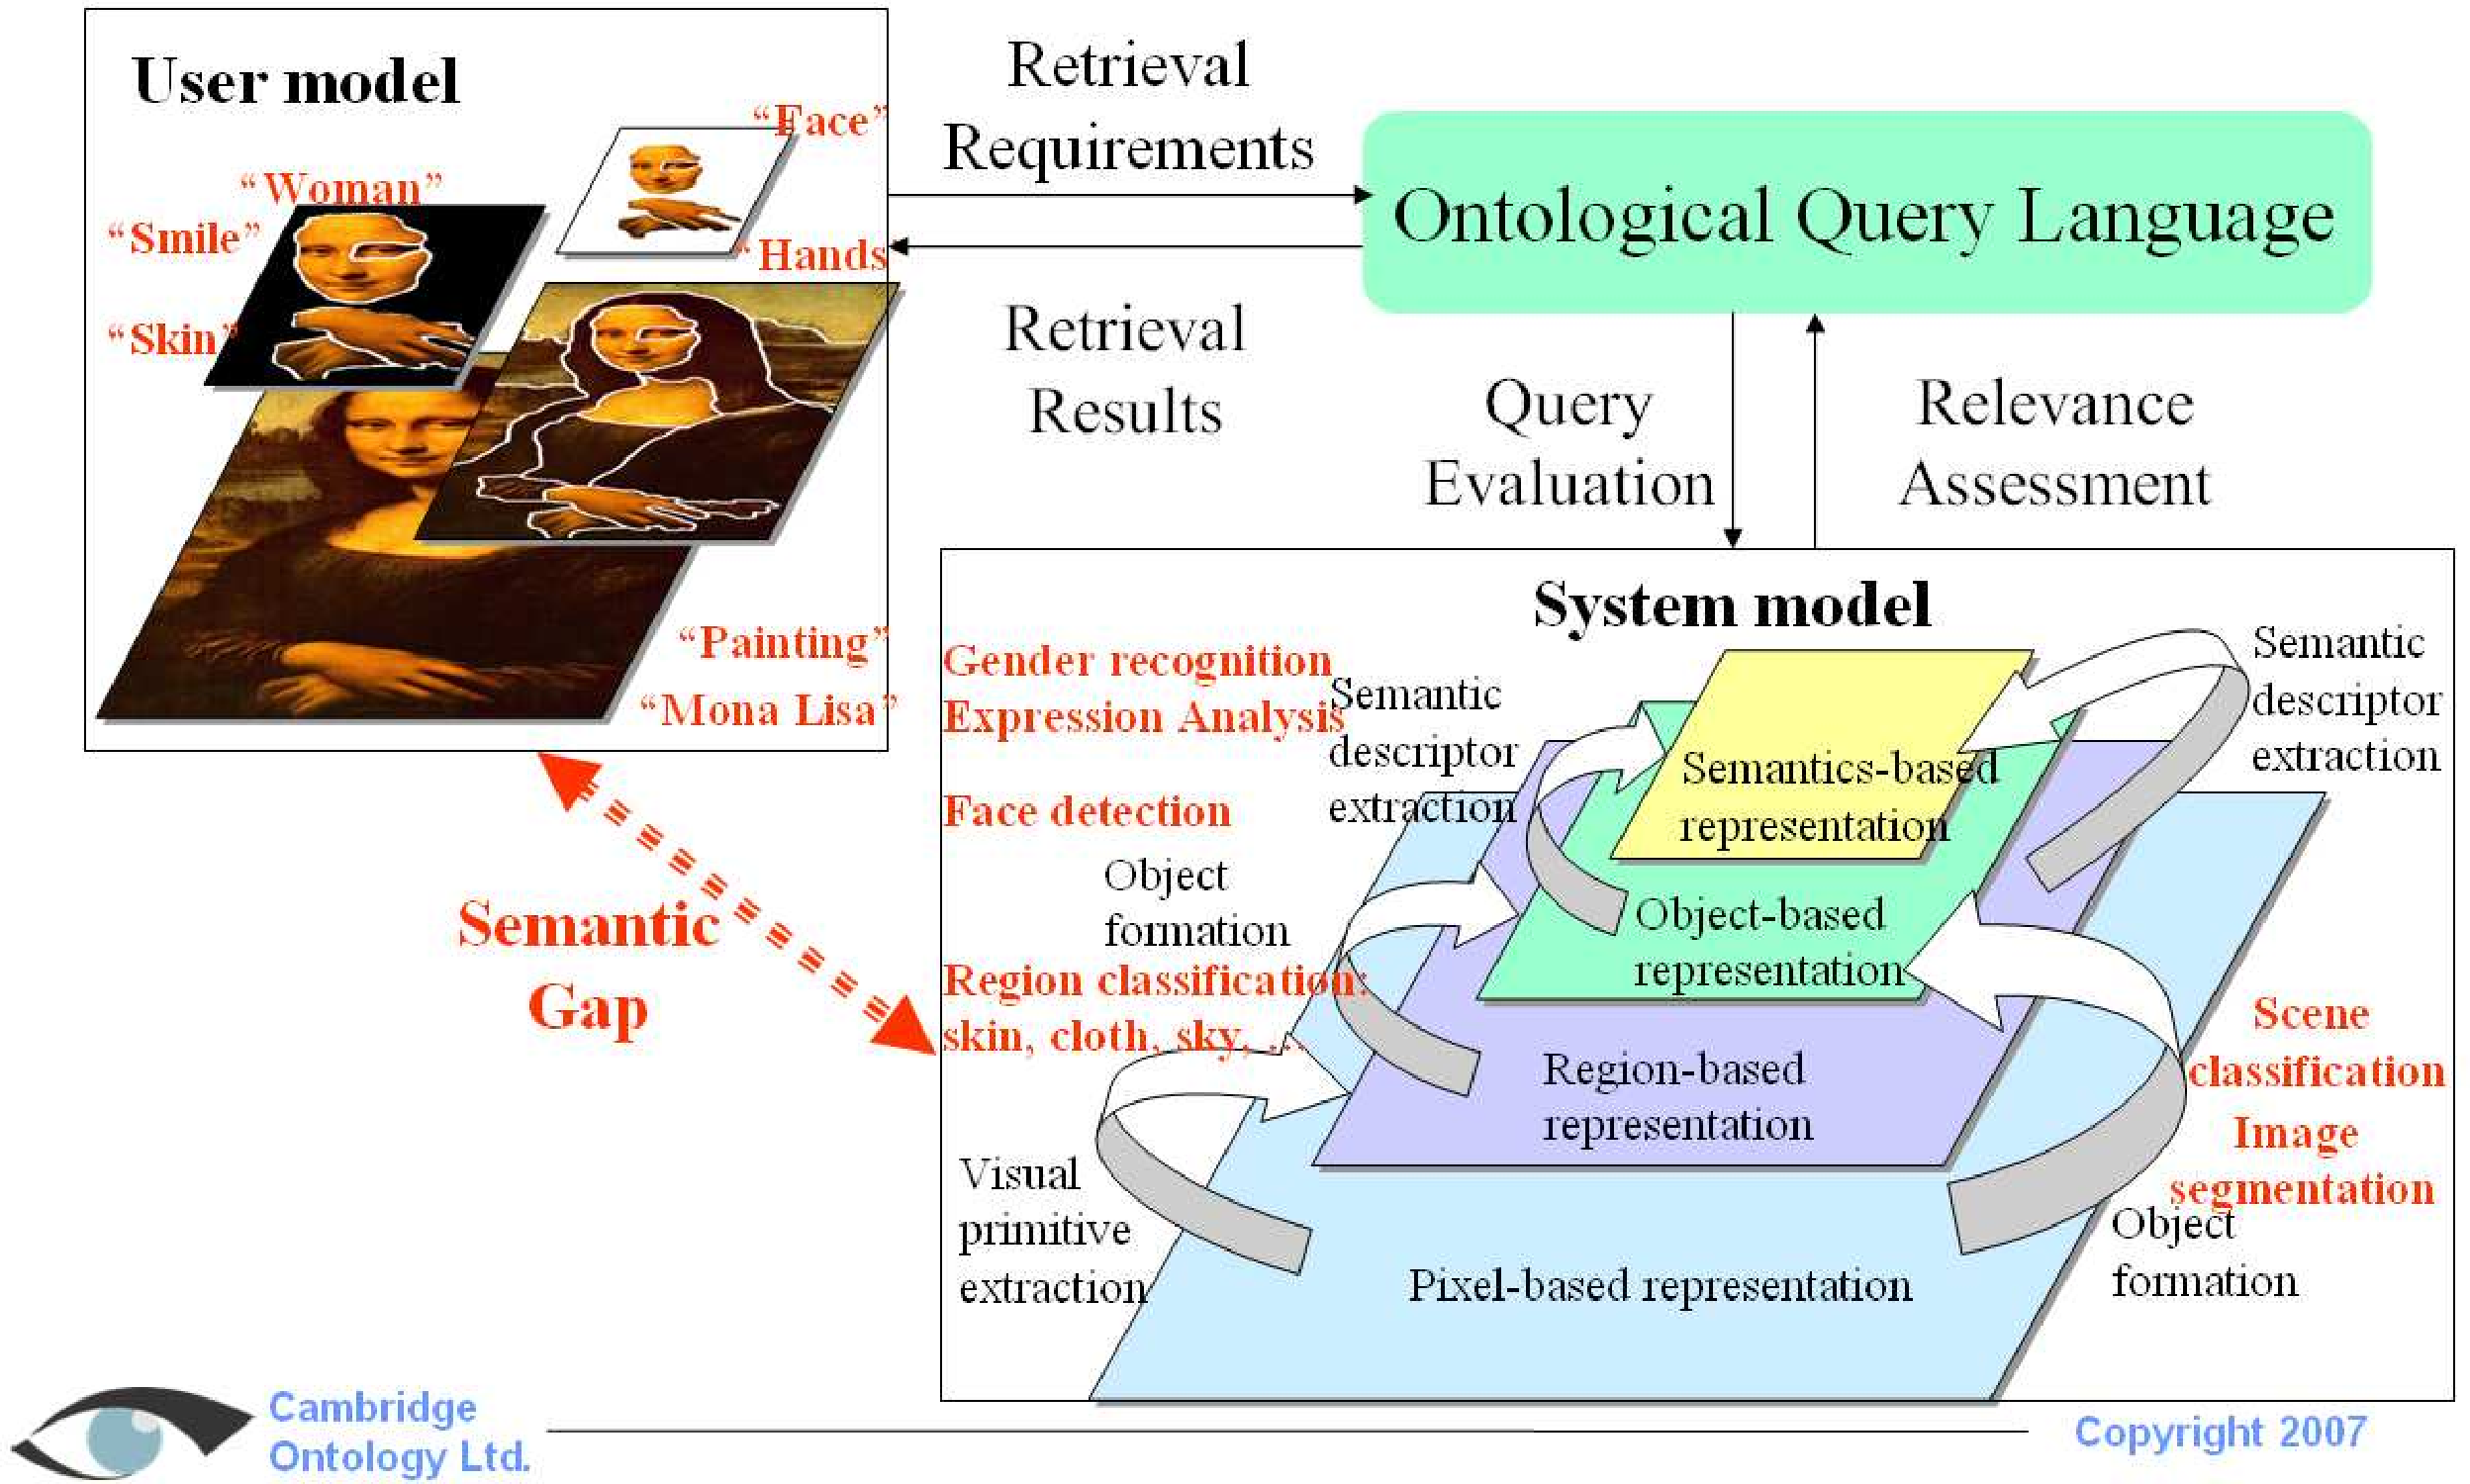
\includegraphics[width=0.85 \textwidth]{camtologytech.eps}
\end{center}
\caption[]{\bf Diagrammatic overview of the image analysis and recognition carried out by Cambridge Ontology Ltd..}
\label{f:camtologytech}
\end{figure}


%%%%%%%%%%%%%%%%%%%%%%%%%%%%%%%%%%%%%%%%%%%%%%%%%%%%%%%%%%%%%%%%%%%%%
%%%%%%%%%%%%%%%%%%%%%%%%%%%%%%%%%%%%%%%%%%%%%%%%%%%%%%%%%%%%%%%%%%%%%
\section{Image Analysis}

The processing stages involved in the image search system, i.e. image analysis and indexing, are intrinsically sequential. In order to benefit from parallelisation, it was decided to parallelise at the granularity of single images or small subsets of images. Each image can therefore be processed in isolation on the Grid, and such processing takes no more than few seconds or tens of seconds on a typical GridPP node. In order to minimise overheads, several hundred images are automatically agglomerated into a batch which is then submitted for processing via GANGA, with the results of image processing and analysis being passed back to the submission server upon successful completion.

As illustrated in figure \ref{f:camtologytech}, Cambridge Ontology's technology comprises a number of complex processing stages in order to analyse the content of an image. While the methods employed are proprietary, the overall process is related to earlier work by the founders of Cambridge Ontology which has been published (see \cite{Town2004, TownPhD}). Broadly speaking, the image analysis consists of the following stages:

\begin{itemize}

\item {\em Image segmentation}: In order to identify salient parts of the image corresponding to objects or object parts, the image is automatically segmented into a covering set of non-overlapping regions and sets of properties such as size, colour, shape, and texture are computed for each region. The number of segmented regions depends on image size and visual complexity, but has the desirable property that most of the image area is usually contained within a few dozen regions which closely correspond to the salient features of the picture.

\item {\em Region classification}: Segmented regions are then automatically classified according to a predefined set of material and environmental categories, such as ``grass'', ``sky'', ``wood'', ``water'' etc.. Sophisticated statistical machine learning methods are employed to yield a highly reliably probabilistic classification of the image. This may be regarded as an intermediate level semantic representation which serves as the basis for subsequent stages of visual inference and composite object recognition.

\item {\em Scene classification}: A second stage of classifiers is applied to analyse image content at a higher scene level. Examples of scene categories include ``indoor'', ``beach'', ``sunset'', ``nighttime'', ``autumn'', etc..

\item {\em Object detection and recognition}: The image analysis also features detectors for common objects. For example, human faces are automatically detected and classified according to personal attributes such as gender, age, and facial expression.

\item {\em Index generation}: Once all image analysis stages have been applied, then all the information from the various classifiers and recognisers is combined into a special indexing format which supports fast content based image retrieval. The searchable index itself is later compiled at a central server, although it may be practical in future to maintain a distributed index across multiple Grid sites to support very large indexes with many millions of images.

\end{itemize}






{\small

\bibliographystyle{plain}
\bibliography{camtologyrefs}

}

\end{document}
